\chapter{Fundamentação Teórica}
\label{cap:revisao}

\section{Dinâmica e Modos de Falha em Rolamentos de Elementos Rolantes}
\label{sec:dinamica_rolamentos}

Os rolamentos de elementos rolantes constituem pares cinemáticos de precisão projetados para suportar carregamentos mecânicos elevados, minimizando as perdas por atrito viscoso e de contato entre componentes em movimento relativo \cite{harris2006rolling}. Em rodeiros e caixas de mancal ferroviárias, a integridade mecânica desses elementos governa a confiabilidade de todo o sistema de tração e sustentação do trem.

Estruturalmente, um rolamento radial típico é composto por quatro elementos fundamentais:
\begin{enumerate}
    \item \textbf{Pista interna (\textit{inner race}):} anel montado solidariamente ao eixo rotativo do rodeiro;
    \item \textbf{Pista externa (\textit{outer race}):} anel fixado ao alojamento estacionário da caixa de mancal (\textit{axlebox});
    \item \textbf{Elementos rolantes (esferas ou rolos):} corpos intermediários que transmitem a carga dinâmica entre os anéis através de áreas de contato hertziano reduzidas;
    \item \textbf{Gaiola espaçadora (\textit{cage}):} estrutura responsável por manter o espaçamento angular uniforme entre os elementos rolantes, prevenindo o contato metal-metal mútuo.
\end{enumerate}

\subsection{Cinemática e Frequências Características de Defeito}
\label{subsec:frequencias_falha}

Quando uma descontinuidade mecânica localizada (como um micropitting, trinca ou cavidade gerada por fadiga de contato) surge em um dos componentes do rolamento, a passagem sucessiva dos elementos rolantes sobre essa superfície danificada gera impactos impulsivos repetitivos de curtíssima duração \cite{randall2011rolling}. A periodicidade temporal desses impactos é estritamente vinculada à cinemática geométrica do rolamento e à rotação do eixo.

Considerando um rolamento operando em regime de contato puro (sem escorregamento cinemático), as frequências cinemáticas fundamentais de repetição dos impactos são deduzidas analiticamente a partir dos parâmetros dimensionais ilustrados na \autoref{fig:geometria_rolamento} \cite{harris2006rolling}:
\begin{itemize}
    \item $d$: diâmetro dos elementos rolantes (esferas ou rolos) [\si{\meter} ou \si{in}];
    \item $D$: diâmetro primitivo ou diâmetro de passo (\textit{pitch diameter}) [\si{\meter} ou \si{in}];
    \item $n$: quantidade de elementos rolantes no conjunto;
    \item $\phi$: ângulo de contato da carga em relação ao plano radial [\si{\degree}];
    \item $f_r$: frequência fundamental de rotação do eixo [\si{\hertz}], calculada a partir da velocidade em rotações por minuto ($\text{RPM}$) por:
    \begin{equation}
        f_r = \frac{\text{RPM}}{60}
        \label{eq:frequencia_rotacao}
    \end{equation}
    onde:
    \begin{itemize}
        \item $f_r$ é a frequência de giro do eixo [\si{\hertz}];
        \item $\text{RPM}$ é a velocidade angular do eixo [\si{rpm}].
    \end{itemize}
\end{itemize}

\begin{figure}[htbp]
    \centering
    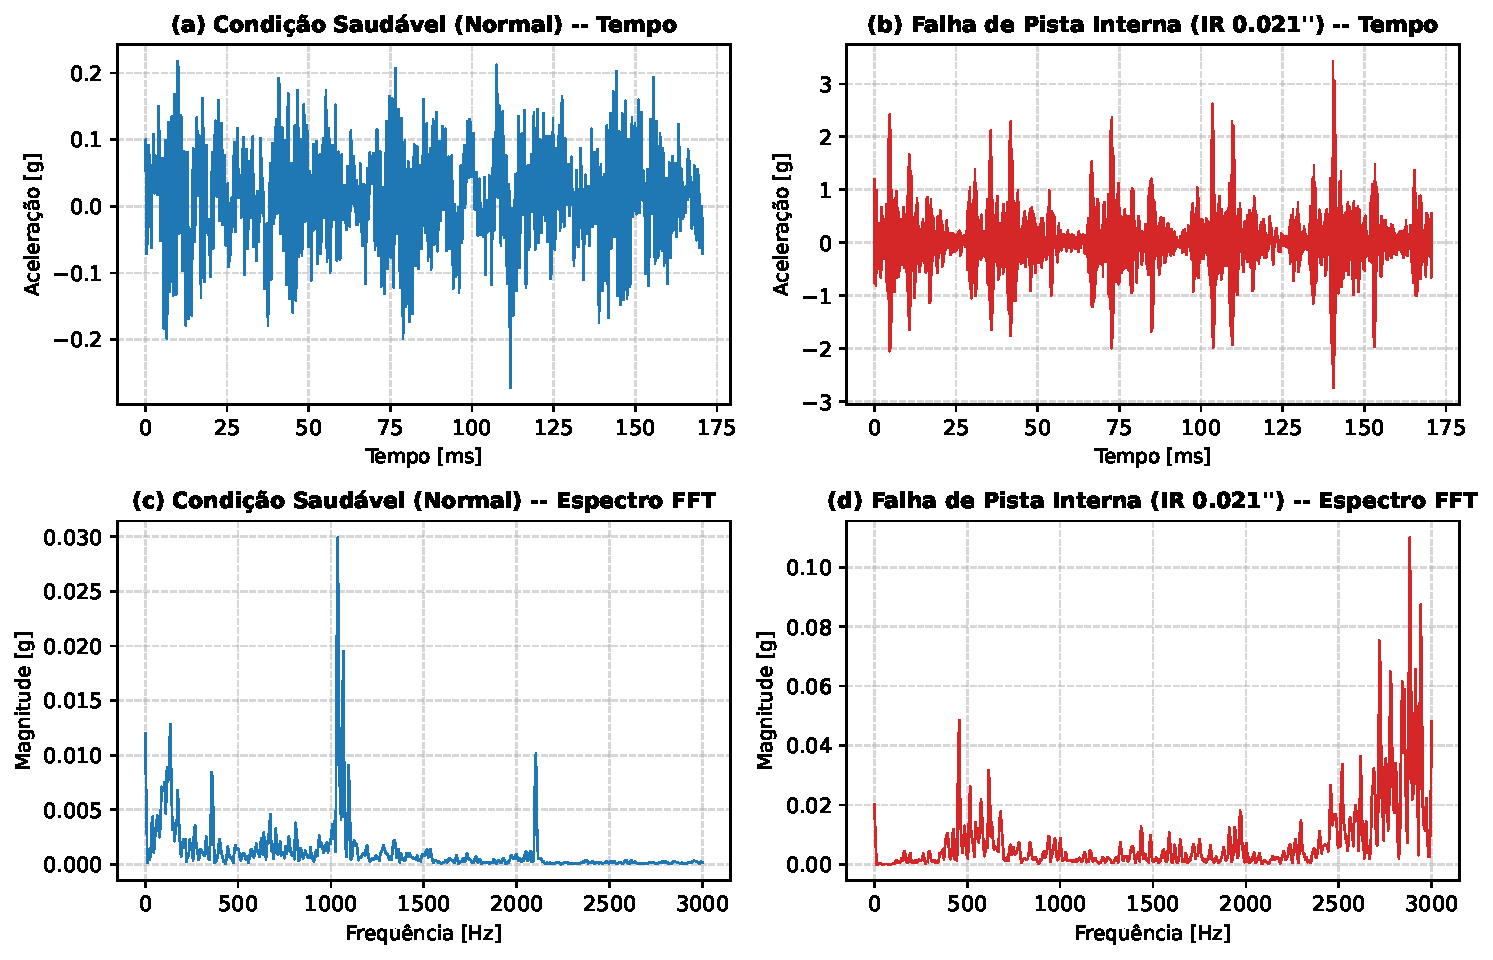
\includegraphics[width=0.55\textwidth]{fig_sinais_tempo_fft.pdf}
    \caption{Representação esquemática dos parâmetros geométricos de um rolamento radial de esferas}
    \label{fig:geometria_rolamento}
    \legend{Fonte: Adaptado de Randall e Antoni (2011).}
\end{figure}

A partir dessas grandezas dimensionais, definem-se quatro frequências características de defeito:

\subsubsection{Frequência de Passagem de Esferas pela Pista Externa (BPFO)}
A frequência BPFO (\textit{Ball Pass Frequency Outer}) corresponde à taxa de repetição dos impactos gerados quando os elementos rolantes transitam sobre um ponto de falha localizado na pista externa estacionária:
\begin{equation}
    \text{BPFO} = \frac{n \cdot f_r}{2} \left( 1 - \frac{d}{D} \cos\phi \right)
    \label{eq:bpfo}
\end{equation}
onde:
\begin{itemize}
    \item $\text{BPFO}$ é a frequência característica de defeito na pista externa [\si{\hertz}];
    \item $n$ é o número de elementos rolantes;
    \item $f_r$ é a rotação do eixo [\si{\hertz}];
    \item $d$ é o diâmetro da esfera [\si{\meter} ou \si{in}];
    \item $D$ é o diâmetro primitivo [\si{\meter} ou \si{in}];
    \item $\phi$ é o ângulo de contato mecânico [\si{\degree}].
\end{itemize}

\subsubsection{Frequência de Passagem de Esferas pela Pista Interna (BPFI)}
A frequência BPFI (\textit{Ball Pass Frequency Inner}) quantifica os impactos decorrentes da passagem dos elementos rolantes sobre um ponto com defeito na pista interna solidária ao eixo rotativo:
\begin{equation}
    \text{BPFI} = \frac{n \cdot f_r}{2} \left( 1 + \frac{d}{D} \cos\phi \right)
    \label{eq:bpfi}
\end{equation}
onde:
\begin{itemize}
    \item $\text{BPFI}$ é a frequência característica de defeito na pista interna [\si{\hertz}], sendo fisicamente superior à $\text{BPFO}$ devido à rotação relativa da pista interna.
\end{itemize}

\subsubsection{Frequência de Giro do Elemento Rolante (BSF)}
A frequência BSF (\textit{Ball Spin Frequency}) representa a rotação própria da esfera em torno do seu próprio centro geométrico. Cada revolução completa da esfera com defeito superficial gera dois impactos sucessivos (um contra a pista interna e outro contra a pista externa):
\begin{equation}
    \text{BSF} = \frac{D \cdot f_r}{2d} \left[ 1 - \left(\frac{d}{D}\cos\phi\right)^2 \right]
    \label{eq:bsf}
\end{equation}
onde:
\begin{itemize}
    \item $\text{BSF}$ é a frequência angular de giro da esfera [\si{\hertz}].
\end{itemize}

\subsubsection{Frequência Fundamental da Gaiola (FTF)}
A frequência FTF (\textit{Fundamental Train Frequency}) expressa a velocidade angular de rotação do conjunto da gaiola que aloja os elementos rolantes em relação ao anel externo estacionário:
\begin{equation}
    \text{FTF} = \frac{f_r}{2} \left( 1 - \frac{d}{D}\cos\phi \right)
    \label{eq:ftf}
\end{equation}
onde:
\begin{itemize}
    \item $\text{FTF}$ é a frequência de revolução do trem de esferas/gaiola [\si{\hertz}].
\end{itemize}

Em rolamentos radiais puros, o ângulo de contato é nulo ($\phi = 0^\circ$), simplificando o termo $\cos\phi = 1,0$ nas \autoref{eq:bpfo} a \ref{eq:ftf}.

\subsection{Mecanismos Físicos de Propagação e Modulação de Vibração}
\label{subsec:modulacao_vibracao}

A detecção de falhas em rolamentos baseada em vibrações envolve aspectos dinâmicos sutis:
\begin{enumerate}
    \item \textbf{Resposta Impulsiva e Ressonância Estrutural:} Os impactos pontuais exercidos pelo defeito comportam-se como trens de impulsos de Dirac no domínio do tempo, possuindo um espectro contínuo de banda larga. Esses impactos excitam as frequências naturais de vibração da carcaça do mancal e do sensor acelerométrico (tipicamente localizadas em faixas de alta frequência, entre \SI{2}{\kilo\hertz} e \SI{10}{\kilo\hertz}) \cite{randall2011rolling};
    \item \textbf{Modulação de Amplitude em Falhas de Pista Interna e Esferas:} Quando a falha situa-se na pista interna, a região danificada gira solidariamente ao eixo, adentrando e saindo periodicamente da zona de carga principal do mancal. Em consequência, a amplitude dos pulsos de vibração gerados na frequência $\text{BPFI}$ sofre modulação em amplitude (\textit{Amplitude Modulation} -- AM) na frequência de rotação do eixo ($f_r$). No domínio da frequência, isso se manifesta pelo surgimento de bandas laterais (\textit{sidebands}) espaçadas de $\pm f_r$ em torno da $\text{BPFI}$ e de seus harmônicos \cite{smith2015rolling};
    \item \textbf{Estacionariedade da Zona de Carga na Pista Externa:} Como a pista externa é estacionária em mancais de rodeiros ferroviários, um defeito centrado no fundo da zona de carga sofrerá impactos de intensidade uniforme a cada passagem de esfera, resultando em menor dispersão por modulação comparativamente às falhas de pista interna.
\end{enumerate}

\section{Processamento Digital de Sinais Aplicado à Análise de Vibrações}
\label{sec:processamento_sinais}

O sinal de vibração discretizado $x[n] = x(n T_s)$ corresponde a uma série temporal de $N$ amostras adquirida a uma taxa de amostragem constante $f_s = 1/T_s$. Para viabilizar a classificação supervisionada por algoritmos de Aprendizado de Máquina, o sinal contínuo deve ser convertido em um conjunto compacto de descritores matemáticos informativos nos domínios do tempo e da frequência \cite{oppenheim2010discrete}.

\subsection{Descritores Estatísticos no Domínio do Tempo}
\label{subsec:features_tempo}

As características no domínio do tempo caracterizam as propriedades estocásticas da série temporal, quantificando energia basal, dispersão e a presença de picos transitórios agudos \cite{antoni2006spectral}:

\subsubsection{Valor Eficaz (Root Mean Square -- RMS)}
O valor RMS quantifica a potência média e a energia cinética global contida no sinal de vibração ao longo da janela:
\begin{equation}
    \text{RMS} = \sqrt{\frac{1}{N} \sum_{i=1}^{N} x_i^2}
    \label{eq:rms}
\end{equation}
onde:
\begin{itemize}
    \item $\text{RMS}$ é o valor eficaz do sinal de aceleração [\si{g} ou \si{\meter\per\second\squared}];
    \item $x_i$ é a $i$-ésima amostra de aceleração discretizada;
    \item $N$ é o número total de pontos na janela de análise.
\end{itemize}

\subsubsection{Curtose (Kurtosis)}
A curtose é o quarto momento estatístico normalizado, constituindo uma métrica sensível à impulsividade do sinal. Valores de curtose próximos a 3 indicam distribuição normal (típica de rolamentos sadios com ruído gaussiano), ao passo que impactos periódicos decorrentes de falhas elevam substancialmente o valor da curtose \cite{antoni2006spectral}:
\begin{equation}
    K = \frac{\frac{1}{N} \sum_{i=1}^{N} (x_i - \bar{x})^4}{\left( \frac{1}{N} \sum_{i=1}^{N} (x_i - \bar{x})^2 \right)^2}
    \label{eq:curtose}
\end{equation}
onde:
\begin{itemize}
    \item $K$ é a curtose adimensional (com convenção de referência em $3,0$ para distribuição gaussiana);
    \item $\bar{x}$ é a média aritmética das amostras da janela.
\end{itemize}

\subsubsection{Fator de Crista (Crest Factor)}
O Fator de Crista expressa a razão entre a amplitude de pico absoluta e a energia média eficaz do sinal, indicando a predominância de choques pontuais em relação ao ruído de fundo:
\begin{equation}
    \text{CF} = \frac{\max_{1 \le i \le N} |x_i|}{\text{RMS}}
    \label{eq:fator_crista}
\end{equation}
onde:
\begin{itemize}
    \item $\text{CF}$ é o fator de crista adimensional ($\text{CF} \ge 1,0$).
\end{itemize}

\subsubsection{Desvio Padrão ($\sigma$)}
O desvio padrão mensura a variabilidade da aceleração em torno da média:
\begin{equation}
    \sigma = \sqrt{\frac{1}{N} \sum_{i=1}^{N} (x_i - \bar{x})^2}
    \label{eq:desvio_padrao}
\end{equation}
onde:
\begin{itemize}
    \item $\sigma$ é o desvio padrão da aceleração [\si{g} ou \si{\meter\per\second\squared}].
\end{itemize}

\subsubsection{Assimetria (Skewness)}
O terceiro momento estatístico quantifica a assimetria da distribuição de probabilidade das amplitudes do sinal em relação à média:
\begin{equation}
    S = \frac{\frac{1}{N} \sum_{i=1}^{N} (x_i - \bar{x})^3}{\sigma^3}
    \label{eq:assimetria}
\end{equation}
onde:
\begin{itemize}
    \item $S$ é o coeficiente de assimetria adimensional.
\end{itemize}

\subsubsection{Valor Pico a Pico (Peak-to-Peak)}
Representa a excursão dinâmica máxima da aceleração instantânea na janela:
\begin{equation}
    X_{p-p} = \max_{1 \le i \le N} (x_i) - \min_{1 \le i \le N} (x_i)
    \label{eq:pico_a_pico}
\end{equation}
onde:
\begin{itemize}
    \item $X_{p-p}$ é a amplitude pico a pico [\si{g} ou \si{\meter\per\second\squared}].
\end{itemize}

\subsubsection{Fator de Forma e Fator de Impulso}
O Fator de Forma ($\text{SF}$) e o Fator de Impulso ($\text{IF}$) relacionam o valor RMS e o valor de pico à média retificada absoluta do sinal, respectivamente:
\begin{equation}
    \text{SF} = \frac{\text{RMS}}{\frac{1}{N} \sum_{i=1}^{N} |x_i|}, \quad \text{IF} = \frac{\max_{1 \le i \le N} |x_i|}{\frac{1}{N} \sum_{i=1}^{N} |x_i|}
    \label{eq:fatores_forma_impulso}
\end{equation}

\subsection{Análise no Domínio da Frequência e Análise de Envelope}
\label{subsec:analise_frequencia}

Embora as estatísticas temporais sejam sensíveis à severidade global do dano, elas não discriminam isoladamente qual componente interno do rolamento está avariado. Essa identificação requer a conversão do sinal para o domínio da frequência por meio da Transformada Discreta de Fourier (\textit{Discrete Fourier Transform} -- DFT) \cite{oppenheim2010discrete}:
\begin{equation}
    X[k] = \sum_{n=0}^{N-1} x[n] \cdot e^{-j \frac{2\pi}{N} k n}, \quad k = 0, 1, \dots, N-1
    \label{eq:dft}
\end{equation}
onde:
\begin{itemize}
    \item $X[k]$ são os coeficientes espectrais complexos na frequência $f_k = k \frac{f_s}{N}$;
    \item $j = \sqrt{-1}$ é a unidade imaginária.
\end{itemize}

Computacionalmente, a DFT é executada mediante o algoritmo da Transformada Rápida de Fourier (\textit{Fast Fourier Transform} -- FFT), reduzindo a complexidade de $\mathcal{O}(N^2)$ para $\mathcal{O}(N \log N)$. 

Para atenuar o fenômeno de espalhamento espectral (\textit{spectral leakage}) provocado pelo truncamento abrupto da janela temporal, aplica-se previamente uma função de janelamento suave, sendo a janela de Hanning a mais consagrada na literatura de vibrações:
\begin{equation}
    w[n] = 0,5 - 0,5 \cos\left( \frac{2\pi n}{N-1} \right), \quad n = 0, 1, \dots, N-1
    \label{eq:hanning}
\end{equation}

\subsubsection{Análise de Envelope via Transformada de Hilbert}
Como destacado na \autoref{subsec:modulacao_vibracao}, as repetições de impacto de baixa frequência ($\text{BPFO}, \text{BPFI}, \text{BSF} < \SI{300}{\hertz}$) modulam em amplitude ressonâncias estruturais de alta frequência ($> \SI{2000}{\hertz}$). Em uma FFT direta, a amplitude nessas frequências baixas pode ficar submersa no ruído basal da máquina \cite{randall2011rolling}.

A Análise de Envelope soluciona essa limitação desmodulando o sinal mediante a construção do sinal analítico complexo $z(t)$ via Transformada de Hilbert $\mathcal{H}\{x(t)\}$:
\begin{equation}
    z(t) = x(t) + j \mathcal{H}\{x(t)\} = x(t) + j \left( \frac{1}{\pi} \text{P.V.} \int_{-\infty}^{\infty} \frac{x(\tau)}{t - \tau} d\tau \right)
    \label{eq:hilbert}
\end{equation}
onde $\text{P.V.}$ denota o Valor Principal de Cauchy da integral imprópria.

O envelope de amplitude instantânea $e(t)$ é definido pela magnitude do sinal analítico:
\begin{equation}
    e(t) = |z(t)| = \sqrt{x^2(t) + [\mathcal{H}\{x(t)\}]^2}
    \label{eq:envelope}
\end{equation}

Como o sinal resultante $e(t)$ é estritamente não negativo, ele carrega um offset de corrente contínua (DC) pronunciado. Para evitar a saturação de energia no bin de \SI{0}{\hertz} da FFT, subtrai-se a média do envelope antes do cálculo espectral:
\begin{equation}
    e_{\text{proc}}(t) = e(t) - \frac{1}{N}\sum_{i=1}^{N} e_i
    \label{eq:envelope_sem_dc}
\end{equation}

A FFT aplicada sobre $e_{\text{proc}}(t)$ revela com clareza os picos espectrais coincidentes com as frequências cinemáticas $\text{BPFO}$, $\text{BPFI}$ e $\text{BSF}$.

\section{Aprendizado de Máquina na Classificação de Falhas}
\label{sec:machine_learning}

\subsection{Classificador Random Forest}
\label{subsec:random_forest}

O algoritmo \textit{Random Forest}, proposto por \citeonline{breiman2001random}, é um método de aprendizado por comitê (\textit{ensemble learning}) fundamentado no princípio do empacotamento estatístico (\textit{bagging} -- \textit{Bootstrap Aggregating}) aplicado a árvores de decisão. 

Em vez de treinar uma única árvore profunda propensa ao sobreajuste (\textit{overfitting}), o modelo constrói uma floresta de $B$ árvores de decisão independentes. Para cada árvore $b \in \{1, \dots, B\}$, seleciona-se uma amostra com reposição do conjunto de treino original. Durante a divisão de cada nó da árvore, avalia-se apenas um subconjunto aleatório de $m \approx \sqrt{p}$ atributos entre os $p$ atributos disponíveis, descorrelacionando os estimadores individuais \cite{breiman2001random}.

A decisão em cada nó é governada pela minimização da impureza de Gini:
\begin{equation}
    I_G(t) = 1 - \sum_{k=1}^{C} p_{t, k}^2
    \label{eq:gini}
\end{equation}
onde:
\begin{itemize}
    \item $I_G(t)$ é o índice de impureza do nó $t$;
    \item $p_{t, k}$ é a proporção de amostras da classe $k \in \{1, \dots, C\}$ presentes no nó $t$.
\end{itemize}

A predição final para uma nova janela de sinal $\mathbf{x}$ é obtida por votação majoritária entre todas as árvores da floresta:
\begin{equation}
    \hat{y} = \arg\max_{c \in \{1, \dots, C\}} \sum_{b=1}^{B} I(h_b(\mathbf{x}) = c)
    \label{eq:votacao_rf}
\end{equation}
onde $h_b(\mathbf{x})$ é o voto emitido pela $b$-ésima árvore. 

O modelo fornece adicionalmente a Importância Média de Redução de Impureza (\textit{Mean Decrease in Impurity} -- MDI), quantificando a contribuição relativa de cada atributo para a pureza da classificação.

\subsection{Support Vector Machines (SVM)}
\label{subsec:svm}

A técnica de Máquinas de Vetores de Suporte (\textit{Support Vector Machines} -- SVM), formalizada por \citeonline{cortes1995support}, busca determinar o hiperplano ótimo em um espaço de características multidimensional que maximize a margem de separação entre as classes de dados.

Dado um conjunto de treinamento $\{(\mathbf{x}_i, y_i)\}_{i=1}^{N}$, com $\mathbf{x}_i \in \mathbb{R}^p$ e rótulos $y_i \in \{-1, +1\}$, a formulação primal com margens suaves (\textit{soft margin}) e penalidade de erro $C > 0$ é expressa pelo problema de programação quadrática convexa:
\begin{equation}
    \min_{\mathbf{w}, b, \boldsymbol{\xi}} \frac{1}{2} \|\mathbf{w}\|^2 + C \sum_{i=1}^{N} \xi_i
    \label{eq:svm_primal}
\end{equation}
sujeito às restrições lineares:
\begin{equation}
    y_i (\mathbf{w}^T \phi(\mathbf{x}_i) + b) \ge 1 - \xi_i, \quad \xi_i \ge 0, \quad \forall i = 1, \dots, N
    \label{eq:svm_restricoes}
\end{equation}
onde:
\begin{itemize}
    \item $\mathbf{w}$ é o vetor normal que orienta o hiperplano divisor;
    \item $b$ é o termo de polarização (\textit{bias});
    \item $\xi_i$ são variáveis de folga que toleram amostras dentro da margem ou mal classificadas;
    \item $C$ é a constante de regularização que equilibra a largura da margem e a penalização por violação de fronteira;
    \item $\phi(\cdot)$ é uma transformação não linear que projeta os dados em um espaço de dimensão superior.
\end{itemize}

Mediante a aplicação das condições de Karush-Kuhn-Tucker (KKT) e a formulação dual de Lagrange, a função de decisão depende exclusivamente de produtos escalares computados eficientemente através de uma função de \textit{kernel} $K(\mathbf{x}_i, \mathbf{x}_j) = \phi(\mathbf{x}_i)^T \phi(\mathbf{x}_j)$ (\textit{kernel trick}) \cite{cortes1995support}. Para padrões vibracionais mecânicos não lineares, o \textit{kernel} Gaussiano de Base Radial (\textit{Radial Basis Function} -- RBF) é o mais recomendado:
\begin{equation}
    K(\mathbf{x}_i, \mathbf{x}_j) = \exp\left( -\gamma \|\mathbf{x}_i - \mathbf{x}_j\|^2 \right)
    \label{eq:kernel_rbf}
\end{equation}
onde $\gamma > 0$ governa o raio de influência das amostras de suporte. Para problemas multiclasse ($C > 2$), o SVM utiliza a estratégia de decomposição Um-contra-Um (\textit{One-vs-One} -- OvO).

\subsection{Métricas de Avaliação Multiclasse}
\label{subsec:metricas_avaliacao}

O desempenho dos classificadores em problemas multiclasse é sintetizado pela Matriz de Confusão, cujas linhas representam as classes verdadeiras do rolamento e cujas colunas representam as predições computadas pelo modelo. A partir das contagens de Verdadeiros Positivos ($\text{VP}$), Falsos Positivos ($\text{FP}$), Falsos Negativos ($\text{FN}$) e Verdadeiros Negativos ($\text{VN}$) para cada classe $k$, computam-se as seguintes métricas fundamentais:
\begin{equation}
    \text{Acurácia Global} = \frac{\sum_{k=1}^{C} \text{VP}_k}{\sum_{k=1}^{C} (\text{VP}_k + \text{FP}_k + \text{FN}_k)}
    \label{eq:acuracia}
\end{equation}
\begin{equation}
    \text{Precisão}_k = \frac{\text{VP}_k}{\text{VP}_k + \text{FP}_k}, \quad \text{Sensibilidade}_k (\textit{Recall}) = \frac{\text{VP}_k}{\text{VP}_k + \text{FN}_k}
    \label{eq:precisao_recall}
\end{equation}
\begin{equation}
    \text{F1-Score}_k = 2 \cdot \frac{\text{Precisão}_k \cdot \text{Sensibilidade}_k}{\text{Precisão}_k + \text{Sensibilidade}_k}
    \label{eq:f1_score}
\end{equation}

A média macro (\textit{Macro Average}) agrega o desempenho equitativo entre todas as condições físicas mecânicas:
\begin{equation}
    \text{F1-Score}_{\text{Macro}} = \frac{1}{C} \sum_{k=1}^{C} \text{F1-Score}_k
    \label{eq:f1_macro}
\end{equation}
garantindo que classes com menor número relativo de janelas não sejam mascaradas pela classe com maior volume amostral.
